\section*{(19\textordfeminine\ aula) --- Momento Angular na MQ}

\subsection*{Momento Angular na Mecânica Clássica}

Essa discussão inicial não se encontra no livro.

Na Mecânica Clássica, quando estudamos o movimento de uma partícula em 3D, aparece naturalmente uma variável dinâmica vetorial chamada Momento Angular:
\begin{equation}
    \vec{L} = \vec{r} \times \vec{p} \qquad \text{ou, em componentes,} \qquad
    \begin{cases}
        L_x = y p_z - z p_y \\
        L_y = z p_x - x p_z \\
        L_z = x p_y - y p_x
    \end{cases}
\label{eq:aula19_L_def}
\end{equation}

Essa variável aparece como quantidade conservada nos problemas de força central, como no problema de Kepler de interação gravitacional entre 2 corpos.

Vimos em um exercício no início do curso que os parênteses de Poisson dessas quantidades obedecem
\begin{equation}
    \boxed{\{L_x, L_y\} = L_z \,; \quad \{L_y, L_z\} = L_x \,; \quad \{L_z, L_x\} = L_y}
\label{eq:aula19_poisson_L}
\end{equation}

Por exemplo,
\begin{align}
    \{L_x, L_y\} &= \{y p_z - z p_y, \; z p_x - x p_z\} \notag \\
    &= \{y p_z, z p_x\} - \{y p_z, x p_z\} - \{z p_y, z p_x\} + \{z p_y, x p_z\}
\label{eq:aula19_exemplo_poisson_1}
\end{align}

Antes de usar a propriedade associativa se recorde que os únicos parênteses não nulos são $\{x, p_x\} = \{y, p_y\} = \{z, p_z\} = 1$, portanto:
\begin{align}
    \{L_x, L_y\} &= y p_x \underbrace{\{p_z, z\}}_{-1} + x p_y \underbrace{\{z, p_z\}}_{1} \notag \\
    &= -y p_x + x p_y = L_z
\label{eq:aula19_exemplo_poisson_2}
\end{align}

Com esses parênteses de Poisson podemos calcular $\{\vec{L}^2, L_x\}$, $\{\vec{L}^2, L_y\}$ e $\{\vec{L}^2, L_z\}$, onde $\vec{L}^2 = L_x^2 + L_y^2 + L_z^2$ (é o módulo ao quadrado do vetor $\vec{L}$).

Veja:
\begin{align}
    \{L_x^2 + L_y^2 + L_z^2, \, L_z\} &= \{L_x^2, L_z\} + \{L_y^2, L_z\} + \{L_z^2, L_z\} \notag \\
    &= 2 L_x \underbrace{\{L_x, L_z\}}_{-L_y} + 2 L_y \underbrace{\{L_y, L_z\}}_{L_x} + 2 L_z \underbrace{\{L_z, L_z\}}_{0} = 0
\label{eq:aula19_L2_Lz_poisson}
\end{align}

Similarmente podemos concluir
\begin{equation}
    \boxed{\{\vec{L}^2, L_x\} = \{\vec{L}^2, L_y\} = \{\vec{L}^2, L_z\} = 0}
\label{eq:aula19_L2_poisson_zero}
\end{equation}

\subsection*{Momento Angular na Mecânica Quântica}

Na MQ definimos os 3 operadores
\begin{equation}
    \hat{L}_x = \hat{Y}\hat{P}_z - \hat{Z}\hat{P}_y \,; \qquad
    \hat{L}_y = \hat{Z}\hat{P}_x - \hat{X}\hat{P}_z \,; \qquad
    \hat{L}_z = \hat{X}\hat{P}_y - \hat{Y}\hat{P}_x
\label{eq:aula19_L_operadores}
\end{equation}

Note que não há ambiguidade na ordem dos operadores pois não aparecem termos como $\hat{X}\hat{P}_x$ ou $\hat{Z}\hat{P}_z$. Naturalmente esses operadores são hermitianos.

Definimos também o operador $\hat{L}^2 = \hat{L}_x^2 + \hat{L}_y^2 + \hat{L}_z^2$, correspondente ao tamanho do vetor clássico $\vec{L}$.

As relações de comutação podem ser obtidas facilmente dos comutadores fundamentais:
\begin{equation}
    [\hat{R}_i, \hat{P}_j] = i\hbar \delta_{ij} \qquad [\hat{R}_i, \hat{R}_j] = [\hat{P}_i, \hat{P}_j] = 0
\label{eq:aula19_comutadores_fundamentais}
\end{equation}
encontro
\begin{equation}
    \boxed{[\hat{L}_x, \hat{L}_y] = i\hbar \hat{L}_z \,; \quad [\hat{L}_y, \hat{L}_z] = i\hbar \hat{L}_x \,; \quad [\hat{L}_z, \hat{L}_x] = i\hbar \hat{L}_y}
\label{eq:aula19_comutadores_L}
\end{equation}
em correspondência com os parênteses de Poisson.

Por exemplo:
\begin{align}
    [\hat{L}_y, \hat{L}_z] &= [\hat{Z}\hat{P}_x - \hat{X}\hat{P}_z, \; \hat{X}\hat{P}_y - \hat{Y}\hat{P}_x] \notag \\
    &= [\hat{Z}\hat{P}_x, \hat{X}\hat{P}_y] - [\hat{Z}\hat{P}_x, \hat{Y}\hat{P}_x] - [\hat{X}\hat{P}_z, \hat{X}\hat{P}_y] + [\hat{X}\hat{P}_z, \hat{Y}\hat{P}_x] \notag \\
\label{eq:aula19_exemplo_comutador_1}
\end{align}
(usando os comutadores fundamentais...)
\begin{equation}
    = \hat{Z}\underbrace{[\hat{P}_x, \hat{X}]}_{-i\hbar}\hat{P}_y + \hat{Y}\underbrace{[\hat{X}, \hat{P}_x]}_{i\hbar}\hat{P}_z = i\hbar(\hat{Y}\hat{P}_z - \hat{Z}\hat{P}_y) = i\hbar \hat{L}_x
\label{eq:aula19_exemplo_comutador_2}
\end{equation}

Similarmente,
\begin{equation}
    [\hat{L}^2, \hat{L}_x] = [\hat{L}^2, \hat{L}_y] = [\hat{L}^2, \hat{L}_z] = 0
\label{eq:aula19_comutador_L2}
\end{equation}
de novo em exata correspondência com os parênteses de Poisson.

Esses comutadores mostram que não é possível encontrar autoestados simultâneos de $\hat{L}_x$, $\hat{L}_y$ e $\hat{L}_z$. Isso é diferente do que acontece com os operadores $\hat{X}$, $\hat{Y}$ e $\hat{Z}$, que comutam e têm $\ket{x,y,z}$ como autovetor comum aos 3 operadores, e com os operadores $\hat{P}_x$, $\hat{P}_y$ e $\hat{P}_z$, que também comutam e têm $\ket{p_x,p_y,p_z}$ como autovetor comum.

Em MQ o vetor $\vec{L}$ nunca pode ser completamente especificado em um estado, isto é, não existem estados do tipo $\ket{\ell_x, \ell_y, \ell_z}$. O melhor que podemos conseguir são autoestados simultâneos de $\hat{L}^2$ e de uma das componentes, normalmente escolhida como sendo $\hat{L}_z$.

\subsection*{Autovalores e Autoestados de $\hat{L}^2$ e $\hat{L}_z$}

Quem são os autovalores/autoestados simultâneos de $\hat{L}^2$ e $\hat{L}_z$?

Isso pode ser respondido, como é feito no livro na seção 12.5, usando operadores de criação e destruição. Veremos isso mais adiante; aqui vou seguir a linha tradicional e transformar as equações de autovalor,
\begin{equation}
    \hat{L}^2 \ket{\alpha} = \alpha \ket{\alpha} \qquad \text{e} \qquad \hat{L}_z \ket{\beta} = \beta \ket{\beta}
\label{eq:aula19_eq_autovalor_abstrata}
\end{equation}
em EDP's. Primeiro o operador $\hat{L}_z$:
\begin{equation}
    \braket{\vec{r}}{\hat{L}_z \beta} = \beta \braket{\vec{r}}{\beta} \,, \quad \text{usando } \hat{L}_z = \hat{X}\hat{P}_y - \hat{Y}\hat{P}_x \,,
\label{eq:aula19_Lz_braket}
\end{equation}
\begin{equation}
    i\hbar \left( y \frac{\partial}{\partial x} - x \frac{\partial}{\partial y} \right) \psi_\beta(\vec{r}) = \beta \, \psi_\beta(\vec{r})
\label{eq:aula19_Lz_EDP_cartesiana}
\end{equation}
onde usei $\bra{\vec{r}}\hat{P}_y\ket{\Psi} = -i\hbar \dfrac{\partial \Psi}{\partial y}$, etc.

\subsection*{Mudança para Coordenadas Esféricas}

Uma vez obtida uma EDP podemos escolher usar outro sistema de coordenadas. O sistema esférico é particularmente útil nos problemas envolvendo os operadores de momento angular. Vamos usar:
\begin{equation}
    \psi_\beta(\vec{r}) = \psi_\beta(r, \theta, \varphi)
\label{eq:aula19_psi_esferica}
\end{equation}

Como escrever $\dfrac{\partial \psi_\beta}{\partial x} = \dfrac{\partial \psi_\beta}{\partial r}\dfrac{\partial r}{\partial x} + \dfrac{\partial \psi_\beta}{\partial \theta}\dfrac{\partial \theta}{\partial x} + \dfrac{\partial \psi_\beta}{\partial \varphi}\dfrac{\partial \varphi}{\partial x}$ em termos de $(r,\theta,\varphi)$?

A correspondência entre as coordenadas cartesianas e esféricas é
\begin{equation}
    x = r \sin\theta \cos\varphi \qquad y = r \sin\theta \sin\varphi \qquad z = r \cos\theta
\label{eq:aula19_coordenadas_esfericas}
\end{equation}

Isso torna fácil calcular a matriz abaixo
\begin{equation}
    \begin{pmatrix}
        \dfrac{\partial x}{\partial r} & \dfrac{\partial x}{\partial \theta} & \dfrac{\partial x}{\partial \varphi} \\[2mm]
        \dfrac{\partial y}{\partial r} & \dfrac{\partial y}{\partial \theta} & \dfrac{\partial y}{\partial \varphi} \\[2mm]
        \dfrac{\partial z}{\partial r} & \dfrac{\partial z}{\partial \theta} & \dfrac{\partial z}{\partial \varphi}
    \end{pmatrix}
    =
    \begin{pmatrix}
        \sin\theta\cos\varphi & r\cos\theta\cos\varphi & -r\sin\theta\sin\varphi \\
        \sin\theta\sin\varphi & r\cos\theta\sin\varphi & r\sin\theta\cos\varphi \\
        \cos\theta & -r\sin\theta & 0
    \end{pmatrix}
\label{eq:aula19_matriz_jacobiana_direta}
\end{equation}

No entanto precisamos de $\dfrac{\partial r}{\partial x}$, $\dfrac{\partial \theta}{\partial x}$, etc. escritos em termos de $(r,\theta,\varphi)$. Você é salvo pela observação de que a matriz de derivadas de que você precisa é a inversa da matriz acima.

Como assim? Chamando $x_1 = x$, $x_2 = y$, $x_3 = z$ e $q_1 = r$, $q_2 = \theta$, $q_3 = \varphi$:

$\dfrac{\partial x_i}{\partial q_j}$ é a matriz que temos.

$\dfrac{\partial q_i}{\partial x_j}$ é a matriz desejada.
\begin{equation}
    \sum_{k=1}^{3} \frac{\partial x_i}{\partial q_k}\frac{\partial q_k}{\partial x_j}
    = \frac{\partial x_i}{\partial q_1}\frac{\partial q_1}{\partial x_j} + \frac{\partial x_i}{\partial q_2}\frac{\partial q_2}{\partial x_j} + \frac{\partial x_i}{\partial q_3}\frac{\partial q_3}{\partial x_j}
    = \frac{\partial x_i}{\partial x_j} = \delta_{ij}
\label{eq:aula19_produto_matrizes}
\end{equation}
(produto das duas matrizes)

\begin{equation}
    \begin{pmatrix}
        \dfrac{\partial r}{\partial x} & \dfrac{\partial r}{\partial y} & \dfrac{\partial r}{\partial z} \\[2mm]
        \dfrac{\partial \theta}{\partial x} & \dfrac{\partial \theta}{\partial y} & \dfrac{\partial \theta}{\partial z} \\[2mm]
        \dfrac{\partial \varphi}{\partial x} & \dfrac{\partial \varphi}{\partial y} & \dfrac{\partial \varphi}{\partial z}
    \end{pmatrix}
    =
    \begin{pmatrix}
        \sin\theta\cos\varphi & \sin\theta\sin\varphi & \cos\theta \\[2mm]
        \dfrac{\cos\theta\cos\varphi}{r} & \dfrac{\cos\theta\sin\varphi}{r} & -\dfrac{\sin\theta}{r} \\[2mm]
        -\dfrac{\sin\varphi}{r\sin\theta} & \dfrac{\cos\varphi}{r\sin\theta} & 0
    \end{pmatrix}
\label{eq:aula19_matriz_jacobiana_inversa}
\end{equation}

Encontro então:
\begin{align}
    \frac{\partial}{\partial x} &= \frac{\partial r}{\partial x}\frac{\partial}{\partial r} + \frac{\partial \theta}{\partial x}\frac{\partial}{\partial \theta} + \frac{\partial \varphi}{\partial x}\frac{\partial}{\partial \varphi}
    = (\sin\theta\cos\varphi)\frac{\partial}{\partial r} + \left(\frac{\cos\theta\cos\varphi}{r}\right)\frac{\partial}{\partial \theta} + \left(\frac{-\sin\varphi}{r\sin\theta}\right)\frac{\partial}{\partial \varphi} \label{eq:aula19_ddx_esferica} \\
    \frac{\partial}{\partial y} &= (\sin\theta\sin\varphi)\frac{\partial}{\partial r} + \left(\frac{\cos\theta\sin\varphi}{r}\right)\frac{\partial}{\partial \theta} + \left(\frac{\cos\varphi}{r\sin\theta}\right)\frac{\partial}{\partial \varphi} \label{eq:aula19_ddy_esferica} \\
    \frac{\partial}{\partial z} &= (\cos\theta)\frac{\partial}{\partial r} + \left(\frac{-\sin\theta}{r}\right)\frac{\partial}{\partial \theta} \label{eq:aula19_ddz_esferica}
\end{align}

\subsection*{Operadores $\hat{L}_x$, $\hat{L}_y$, $\hat{L}_z$ em Coordenadas Esféricas}

Com isso podemos obter a ação dos operadores $\hat{L}_x$, $\hat{L}_y$ e $\hat{L}_z$ quando a função de onda está escrita em termos de coordenadas cartesianas ou esféricas.
\begin{align}
    \bra{\vec{r}}\hat{L}_x\ket{\Psi} &= i\hbar\left( z\frac{\partial}{\partial y} - y\frac{\partial}{\partial z} \right)\Psi
    = i\hbar\left( \sin\varphi \frac{\partial}{\partial \theta} + \cot\theta\cos\varphi\frac{\partial}{\partial \varphi} \right)\Psi \label{eq:aula19_Lx_esferica} \\
    \bra{\vec{r}}\hat{L}_y\ket{\Psi} &= i\hbar\left( x\frac{\partial}{\partial z} - z\frac{\partial}{\partial x} \right)\Psi
    = i\hbar\left( -\cos\varphi \frac{\partial}{\partial \theta} + \cot\theta\sin\varphi\frac{\partial}{\partial \varphi} \right)\Psi \label{eq:aula19_Ly_esferica} \\
    \bra{\vec{r}}\hat{L}_z\ket{\Psi} &= i\hbar\left( y\frac{\partial}{\partial x} - x\frac{\partial}{\partial y} \right)\Psi
    = i\hbar\left( -\frac{\partial}{\partial \varphi} \right)\Psi \label{eq:aula19_Lz_esferica}
\end{align}

Essas relações são análogas às relações $\bra{\vec{r}}\hat{P}_z\ket{\Psi} = -i\hbar \dfrac{\partial \Psi}{\partial z}$ para os operadores associados ao momento linear.

De volta à EDP de autovalor do operador $\hat{L}_z$:
\begin{equation}
    \bra{\vec{r}}\hat{L}_z\ket{\beta} = \beta\braket{\vec{r}}{\beta}
    \quad \Longrightarrow \quad
    -i\hbar \frac{\partial}{\partial \varphi}\psi_\beta = \beta \, \psi_\beta
\label{eq:aula19_Lz_autovalor_EDP}
\end{equation}

solução geral (função qualquer):
\begin{equation}
    \psi_\beta(r,\theta,\varphi) = f(r,\theta) \, e^{i\beta\varphi/\hbar}
\label{eq:aula19_Lz_solucao_geral}
\end{equation}

\subsection*{Quantização de $L_z$}

Isso quer dizer que o autovalor $\beta$ pode valer qualquer coisa? \textbf{NÃO!} As funções $\braket{\vec{r}}{\Psi}$ devem associar um único número complexo a cada ponto $\vec{r}$ (isto é, devem ser \textbf{UNÍVOCAS}). Isso acarreta, em particular, que:
\begin{equation}
    \psi_\beta(r,\theta,\varphi+2\pi) = \psi_\beta(r,\theta,\varphi)
\label{eq:aula19_univocidade}
\end{equation}

Isso só acontecerá caso
\begin{equation}
    \beta = m\hbar \qquad (m = 0, \pm 1, \pm 2, \dots)
\label{eq:aula19_beta_quantizado}
\end{equation}

\textbf{Conclusão:} As autofunções do operador $\hat{L}_z$ têm a forma
\begin{equation}
    \boxed{\psi_m = f(r,\theta) \, e^{im\varphi} \qquad (m = 0, \pm 1, \pm 2, \dots)}
\label{eq:aula19_autofuncoes_Lz}
\end{equation}
e correspondem ao autovalor $\boxed{\hbar m}$.

\begin{itemize}
    \item Se você acha estranho não termos conseguido determinar completamente a autofunção, pense no caso das autofunções do operador $\hat{P}_y$, por exemplo
    \begin{equation}
        \bra{\vec{r}}\hat{P}_y\ket{\Psi} = p\braket{\vec{r}}{\Psi}
        \quad \Longrightarrow \quad
        -i\hbar \frac{\partial \Psi}{\partial y} = p\,\Psi
        \quad \Longrightarrow \quad
        \Psi = f(x,z)\, e^{ipy/\hbar}
    \label{eq:aula19_Py_autofuncao}
    \end{equation}
    \item Diferentemente de $\hat{X}, \hat{Y}, \hat{Z}, \hat{P}_x, \hat{P}_y$ e $\hat{P}_z$, ao medir $\hat{L}_z$ só podemos encontrar $\{0, \pm\hbar, \pm2\hbar, \dots\}$: a componente $z$ do momento angular é \textbf{QUANTIZADA}! (Obviamente isso acontece também com $\hat{L}_x$ e $\hat{L}_y$).
\end{itemize}

\subsection*{Autovalores e Autofunções de $\hat{L}^2$}

Com as autofunções de $\hat{L}_z$ determinadas, vamos agora encontrar as autofunções/autovalores de $\hat{L}^2$.

Para determinarmos o que é $\bra{\vec{r}}\hat{L}^2\ket{\Psi}$ usamos $\hat{L}^2 = \hat{L}_x^2 + \hat{L}_y^2 + \hat{L}_z^2$ juntamente com a expressão desses operadores em termos das coordenadas esféricas.
\begin{equation}
    \bra{\vec{r}}\hat{L}^2\ket{\Psi} = (-\hbar^2)\left[ \frac{\partial^2}{\partial \theta^2} + \cot\theta \frac{\partial}{\partial \theta} + \frac{1}{\sin^2\theta}\frac{\partial^2}{\partial \varphi^2} \right]\Psi
\label{eq:aula19_L2_esferica}
\end{equation}

No problema de autovalor para $\hat{L}^2$ vamos admitir que a autofunção de $\hat{L}^2$ é também autofunção de $\hat{L}_z$.
\begin{equation}
    \bra{\vec{r}}\hat{L}^2\ket{\alpha m} = \alpha \braket{\vec{r}}{\alpha m}
\label{eq:aula19_L2_autovalor_alpha}
\end{equation}
onde $\braket{\vec{r}}{\alpha m} = f_{\alpha m}(r,\theta)\, e^{im\varphi}$ é autofunção de $\hat{L}_z$.
\begin{equation}
    (-\hbar^2)\left[ \frac{\partial^2}{\partial \theta^2} + \cot\theta \frac{\partial}{\partial \theta} - \frac{m^2}{\sin^2\theta} \right] f_{\alpha m}(r,\theta) = \alpha \, f_{\alpha m}(r,\theta)
\label{eq:aula19_L2_EDP_theta}
\end{equation}

Podemos escrever $f_{\alpha m}(r,\theta) = R(r)\, P_{\alpha m}(\cos\theta)$, a EDO obedecida por $P_{\alpha m}(x)$ é (função qualquer)
\begin{equation}
    (1-x^2)P_{\alpha m}'' - 2x P_{\alpha m}' - \frac{m^2}{1-x^2}P_{\alpha m} = \left(\frac{\alpha}{-\hbar^2}\right)P_{\alpha m}
\label{eq:aula19_EDO_legendre_generica}
\end{equation}

Essa EDO de 2\textsuperscript{a} ordem pode ser resolvida (a princípio) PARA QUALQUER VALOR DE $\alpha$.

\subsection*{Equação Diferencial Associada de Legendre}

No entanto observe que $-1 \leq x \leq 1$, pois $x = \cos\theta$ e $0 \leq \theta \leq \pi$. Devemos exigir que a função $P_{\alpha m}(x)$ seja regular em $x=1$ e $x=-1$; isso só acontece se
\begin{equation}
    \frac{\alpha}{\hbar^2} = \ell(\ell+1) \qquad (\ell = |m|, |m|+1, |m|+2, \dots)
\label{eq:aula19_alpha_quantizado}
\end{equation}

Nesse caso a equação se chama \textbf{EQUAÇÃO DIFERENCIAL ASSOCIADA DE LEGENDRE} e sua solução geral é
\begin{equation}
    A\, P_\ell^{|m|}(x) + B\, Q_\ell^{|m|}(x)
\label{eq:aula19_solucao_legendre_geral}
\end{equation}

onde $P_\ell^{|m|}(x)$ é a Função Associada de Legendre de 1\textsuperscript{a} classe e $Q_\ell^{|m|}(x)$ é a de 2\textsuperscript{a} classe. Essa última é singular em $x=\pm1$; as autofunções de $\hat{L}^2$ e $\hat{L}_z$ são portanto
\begin{equation}
    \psi_{\ell m}(\vec{r}) = R(r)\, P_\ell^{|m|}(\cos\theta)\, e^{im\varphi}
\label{eq:aula19_autofuncoes_L2_Lz}
\end{equation}

com autovalores $\hbar m$ (para $\hat{L}_z$) e $\hbar^2 \ell(\ell+1)$ (para $\hat{L}^2$).

Os números quânticos $\ell$ e $m$ não são independentes.
\begin{equation}
    m = 0, \pm1, \pm2, \dots \qquad \text{e} \qquad \ell = |m|, |m|+1, \dots
\label{eq:aula19_quantizacao_lm}
\end{equation}

Ambos são inteiros mas $\ell \geq |m|$. Ou seja, para um $\ell$ fixo os valores possíveis de $m$ são $(-\ell, -\ell+1, \dots, \ell-1, \ell)$.

\begin{align}
    P_0^0(x) &= 1 & P_1^0(x) &= x & P_2^0(x) &= \frac{1}{2}(3x^2-1) \notag \\
    P_1^1(x) &= \sqrt{1-x^2} & P_2^1(x) &= 3x\sqrt{1-x^2} & P_2^2(x) &= 3(1-x^2)
\label{eq:aula19_tabela_legendre}
\end{align}

\begin{quote}
\textbf{Observe que} $Y_\ell^{-m}(\theta,\varphi) = (-1)^m \left[ Y_\ell^m(\theta,\varphi) \right]^*$
\end{quote}

Essas funções têm a propriedade
\begin{equation}
    \boxed{\int_{-1}^{1} P_\ell^{|m|}(x)\, P_{\ell'}^{|m|}(x)\, dx = \frac{2}{2\ell+1}\frac{(\ell+|m|)!}{(\ell-|m|)!}\,\delta_{\ell\ell'}}
\label{eq:aula19_ortogonalidade_legendre}
\end{equation}

\subsection*{Harmônicos Esféricos}

A parte angular NORMALIZADA da autofunção de $\hat{L}^2$ e $\hat{L}_z$ se chama \textbf{HARMÔNICO ESFÉRICO}. Sua definição:
\begin{equation}
    \boxed{Y_\ell^m(\theta,\varphi) = \sqrt{\frac{2\ell+1}{2}\frac{(\ell-|m|)!}{(\ell+|m|)!}} \, P_\ell^{|m|}(\cos\theta) \, \frac{e^{im\varphi}}{\sqrt{2\pi}} \times
    \begin{cases}
        (-1)^m, & \text{se } m \geq 0 \\
        1, & \text{se } m < 0
    \end{cases}}
\label{eq:aula19_harmonico_esferico_def}
\end{equation}

Como $\psi_{\ell m}(\vec{r}) = R(r)\, Y_\ell^m(\theta,\varphi)$, a parte radial (arbitrária) da autofunção pode ser normalizada independentemente de $Y_\ell^m(\theta,\varphi)$.
\begin{align}
    \int \psi_{\ell m}^*(\vec{r})\, \psi_{\ell m}(\vec{r}) \, d\vec{r}
    &= \int_0^\infty \int_0^\pi \int_0^{2\pi} |R(r)|^2 \, |Y_\ell^m(\theta,\varphi)|^2 \, r^2 \sin\theta \, dr\, d\theta\, d\varphi \label{eq:aula19_normalizacao_1} \\
    &= \left[ \int_0^\infty |R(r)|^2 r^2 \, dr \right]
    \left[ \underbrace{\frac{2\ell+1}{2}\frac{(\ell-|m|)!}{(\ell+|m|)!} \int_{-1}^{1} \left(P_\ell^{|m|}(x)\right)^2 dx}_{1}
    \underbrace{\int_0^{2\pi} \frac{d\varphi}{2\pi}}_{1} \right] \notag \\
    &= \int_0^\infty |R|^2 r^2 \, dr
\label{eq:aula19_normalizacao_2}
\end{align}
onde usei $\displaystyle\int_0^\pi f(\theta)\sin\theta\, d\theta = \int_{-1}^{1} f(x)\, dx \quad (x=\cos\theta)$.

Alguns harmônicos esféricos:
\begin{align}
    Y_0^0(\theta,\varphi) &= \frac{1}{\sqrt{4\pi}} \notag \\
    Y_1^0(\theta,\varphi) &= \sqrt{\frac{3}{4\pi}}\cos\theta \notag \\
    Y_1^{\pm1}(\theta,\varphi) &= \mp\sqrt{\frac{3}{8\pi}}\sin\theta\, e^{\pm i\varphi} \notag \\
    Y_2^0(\theta,\varphi) &= \sqrt{\frac{5}{16\pi}}\,(3\cos^2\theta - 1) \notag \\
    Y_2^{\pm1}(\theta,\varphi) &= \mp\sqrt{\frac{15}{8\pi}}\cos\theta\sin\theta\, e^{\pm i\varphi} \notag \\
    Y_2^{\pm2}(\theta,\varphi) &= \sqrt{\frac{15}{32\pi}}\sin^2\theta\, e^{\pm i2\varphi}
\label{eq:aula19_tabela_harmonicos}
\end{align}

\subsection*{Distribuição Angular de Probabilidade}

$|Y_\ell^m(\theta,\varphi)|^2$ indica a distribuição angular de probabilidade de uma função de onda do tipo $\Psi(\vec{r}) = R(r)\, Y_\ell^m(\theta,\varphi)$. É comum representar essa função com uma superfície no espaço 3D onde a distância à origem em uma certa direção $(\theta,\varphi)$ corresponde a $|Y_\ell^m(\theta,\varphi)|^2$. Como $|Y_\ell^m|^2$ não depende de $\varphi$, todas as superfícies são superfícies de revolução em torno do eixo-$z$. Basta representar a curva geradora da superfície (gire a curva em torno do eixo-$z$ para obter a superfície).

A seguir, as curvas geradoras (no plano que contém o eixo $z$) dos gráficos polares de $|Y_\ell^m(\theta,\varphi)|^2$ para $\ell = 0, 1, 2$:

\begin{center}
\begin{tikzpicture}[scale=0.9]
    \draw[->] (0,-1.3) -- (0,1.6) node[above] {$z$};
    \draw[->] (-0.2,0) -- (2.2,0);
    \draw (0,0) circle (1.1);
    \node at (2.6,0.6) {$|Y_0^0|^2 = \dfrac{1}{4\pi}$};
\end{tikzpicture}
\end{center}

\begin{center}
\begin{tikzpicture}[scale=0.9]
    \draw[->] (0,-1.8) -- (0,1.8) node[above] {$z$};
    \draw[->] (-1.6,0) -- (1.6,0);
    \draw (0,0.65) circle (0.65);
    \draw (0,-0.65) circle (0.65);
    \node at (3.0,0.9) {$|Y_1^0|^2 = \dfrac{3}{4\pi}\cos^2\theta$};
\end{tikzpicture}
\hspace{1cm}
\begin{tikzpicture}[scale=0.9]
    \draw[->] (0,-1.3) -- (0,1.3) node[above] {$z$};
    \draw[->] (-2,0) -- (2,0);
    \draw (0.7,0) circle (0.7);
    \draw (-0.7,0) circle (0.7);
    \node at (0,-1.6) {$|Y_1^{\pm1}|^2 = \dfrac{3}{8\pi}\sin^2\theta$};
\end{tikzpicture}
\end{center}

\begin{center}
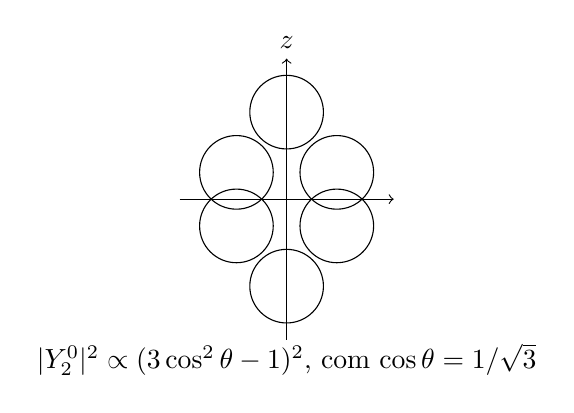
\begin{tikzpicture}[scale=0.85]
    \draw[->] (0,-2.1) -- (0,2.1) node[above] {$z$};
    \draw[->] (-1.6,0) -- (1.6,0);
    \draw (0,1.3) circle (0.55);
    \draw (0,-1.3) circle (0.55);
    \draw (0.75,0.4) circle (0.55);
    \draw (-0.75,0.4) circle (0.55);
    \draw (0.75,-0.4) circle (0.55);
    \draw (-0.75,-0.4) circle (0.55);
    \node at (0,-2.4) {$|Y_2^0|^2 \propto (3\cos^2\theta-1)^2$, com $\cos\theta = 1/\sqrt{3}$};
\end{tikzpicture}
\hspace{0.5cm}
\begin{tikzpicture}[scale=0.85]
    \draw[->] (0,-1.7) -- (0,1.7) node[above] {$z$};
    \draw[->] (-1.6,0) -- (1.6,0);
    \draw (0.7,0.7) circle (0.55);
    \draw (-0.7,0.7) circle (0.55);
    \draw (0.7,-0.7) circle (0.55);
    \draw (-0.7,-0.7) circle (0.55);
    \node at (0,-2.0) {$|Y_2^{\pm1}|^2 = \dfrac{15}{8\pi}\cos^2\theta\sin^2\theta$};
\end{tikzpicture}
\hspace{0.5cm}
\begin{tikzpicture}[scale=0.85]
    \draw[->] (0,-1.3) -- (0,1.3) node[above] {$z$};
    \draw[->] (-1.8,0) -- (1.8,0);
    \draw (1.1,0) circle (0.65);
    \draw (-1.1,0) circle (0.65);
    \node at (0,-1.6) {$|Y_2^{\pm2}|^2 = \dfrac{15}{32\pi}\sin^4\theta$};
\end{tikzpicture}
\end{center}
